\chapter{Mecánica hamiltoniana}\label{ch:b3:hamiltonian-mechanics}

Fotografíese un péndulo mil veces y represéntese, para cada instantánea, su
ángulo frente a su momento angular: los puntos caen sobre una curva cerrada,
y todo movimiento posible del péndulo es una de esas curvas --- las
oscilaciones pequeñas sobre óvalos encajados, las vueltas completas sobre
líneas onduladas por encima y por debajo, y entre ambas una única curva
cruzada que separa los dos regímenes. Esta imagen, el \emph{\omterm{def:b3:hamiltonian-mechanics:portrait}{retrato de
fases}}, es el corazón de la reformulación que Hamilton dio a la mecánica en
1833: el estado de un sistema es un punto del espacio de las coordenadas
\emph{y} de los momentos, su evolución es un flujo en ese espacio, y ese
flujo lo genera una sola función, la energía, mediante dos ecuaciones de
primer orden bellamente simétricas. La recompensa no son cálculos más
fáciles --- ahí suele ganar Lagrange ---, sino la \emph{geometría} correcta:
el flujo conserva el volumen del \omterm{def:b3:hamiltonian-mechanics:hamiltonian}{espacio de fases}, lo que fundará la física
estadística; y su esqueleto algebraico, el \omterm{def:b3:hamiltonian-mechanics:poisson}{corchete de Poisson}, es
justamente lo que la mecánica cuántica promoverá a conmutador. Este capítulo
es la bisagra entre la mecánica de las cosas y la física del siglo XX.

\section{De Lagrange a Hamilton}

\begin{definition}[Hamiltoniano y ecuaciones canónicas]\label{def:b3:hamiltonian-mechanics:hamiltonian}
\index{hamiltoniano}\index{ecuaciones canónicas}\index{espacio de fases}
Para un sistema de \omterm{def:b3:lagrangian-mechanics:action}{lagrangiano} $L(q, \dot q, t)$, exprésense las velocidades
en función de los momentos $p_i = \partial L/\partial\dot q_i$ y defínase
el \emph{hamiltoniano} como la transformada de Legendre
\[
H(q, p, t) = \sum_i p_i\dot q_i - L ,
\]
una función de las coordenadas y de los \emph{momentos}. El espacio de
dimensión $2n$ de los $(q_1, \dots, q_n, p_1, \dots, p_n)$ es el
\emph{espacio de fases}; un punto suyo --- un \emph{estado} --- determina
todo el futuro y todo el pasado del sistema a través de las
\emph{ecuaciones canónicas} del
\cref{thm:b3:hamiltonian-mechanics:canonical}.
\end{definition}

\begin{theorem}[Ecuaciones de Hamilton]\label{thm:b3:hamiltonian-mechanics:canonical}
Las \omterm{thm:b3:lagrangian-mechanics:euler-lagrange}{ecuaciones de Euler--Lagrange} equivalen a las $2n$ ecuaciones de primer
orden
\[
\dot q_i = \frac{\partial H}{\partial p_i} , \qquad
\dot p_i = -\frac{\partial H}{\partial q_i} .
\]
\end{theorem}

\begin{proof}
Derívese $H = \sum p_i\dot q_i - L$ como función de $(q, p, t)$:
$\dd H = \sum(\dot q_i\,\dd p_i + p_i\,\dd\dot q_i) - \sum(
\partial_{q_i}L\,\dd q_i + \partial_{\dot q_i}L\,\dd\dot q_i) -
\partial_tL\,\dd t$. Los términos en $\dd\dot q_i$ se cancelan por la
definición de $p_i$ --- todo el sentido de la transformada de Legendre ---,
lo que deja $\dd H = \sum(\dot q_i\,\dd p_i - \partial_{q_i}L\,\dd q_i) -
\partial_tL\,\dd t$. Leyendo las derivadas parciales:
$\partial H/\partial p_i = \dot q_i$ y $\partial H/\partial q_i =
-\partial L/\partial q_i$, que por Euler--Lagrange vale $-\dot p_i$.
(Además, $\partial_tH = -\partial_tL$).
\end{proof}

\begin{proposition}[Qué es $H$]\label{prop:b3:hamiltonian-mechanics:energy}
$H$ coincide con la \omterm{prop:b3:lagrangian-mechanics:energy}{función energía} $h$ del capítulo anterior: a lo largo de
un movimiento, $\dd H/\dd t = \partial H/\partial t$, de modo que $H$ se
conserva siempre que no dependa explícitamente del tiempo; y cuando la
energía cinética es cuadrática en las velocidades con \omterm{def:b3:lagrangian-mechanics:coordinates}{ligaduras}
independientes del tiempo, $H = E_k + E_p$, la energía mecánica --- escrita
ahora en las variables $(q, p)$.
\end{proposition}

\begin{proof}
$\dd H/\dd t = \sum(\partial_{q_i}H\,\dot q_i + \partial_{p_i}H\,\dot
p_i) + \partial_tH = \sum(\partial_{q_i}H\,\partial_{p_i}H -
\partial_{p_i}H\,\partial_{q_i}H) + \partial_tH = \partial_tH$: la
simetría de las \omterm{def:b3:hamiltonian-mechanics:hamiltonian}{ecuaciones canónicas} hace que la suma se cancele
idénticamente. La identificación con $E_k + E_p$ es la
\cref{prop:b3:lagrangian-mechanics:energy}.
\end{proof}

\begin{example}[Dos hamiltonianos]\label{ex:b3:hamiltonian-mechanics:examples}
Masa sujeta a un resorte: $p = m\dot x$, luego
\[
H = \frac{p^2}{2m} + \frac12 kx^2 ;
\]
las \omterm{def:b3:hamiltonian-mechanics:hamiltonian}{ecuaciones canónicas} $\dot x = p/m$, $\dot p = -kx$ son la pareja
conocida. Péndulo: $p = m\ell^2\dot\theta$ y
\[
H = \frac{p^2}{2m\ell^2} - mg\ell\cos\theta .
\]
En ambos casos $H$ es la energía, constante en cada movimiento: los
movimientos \emph{son} las curvas de nivel de $H$ en el plano $(q,p)$.
\end{example}

\begin{method}[La receta hamiltoniana]\label{met:b3:hamiltonian-mechanics:recipe}
(1) A partir de $L$, calcular los momentos $p_i = \partial L/\partial\dot q_i$
e invertir para obtener las $\dot q_i$. (2) $H = \sum p_i\dot q_i - L$,
expresado solo en $(q, p)$ --- para un sistema natural, simplemente
$E_k + E_p$ con $E_k$ reescrita en los momentos. (3) Escribir las
\omterm{def:b3:hamiltonian-mechanics:hamiltonian}{ecuaciones canónicas}. (4) Dibujar las curvas de nivel de $H$: para un grado
de libertad son las trayectorias, y todo el movimiento cualitativo
--- oscilaciones, rotaciones, equilibrios, separatrices --- se lee sin
resolver nada.
\end{method}

\section{El espacio de fases}

\begin{definition}[Retrato de fases, puntos fijos, separatriz]\label{def:b3:hamiltonian-mechanics:portrait}
\index{retrato de fases}\index{punto fijo}\index{separatriz}
El \emph{retrato de fases} de un sistema es la familia de sus
trayectorias en el \omterm{def:b3:hamiltonian-mechanics:hamiltonian}{espacio de fases}. Un \emph{punto fijo} es un estado en el
que se anulan las dos \omterm{def:b3:hamiltonian-mechanics:hamiltonian}{ecuaciones canónicas} --- un equilibrio: un mínimo del
potencial aparece como un \emph{centro} rodeado de curvas cerradas, y un
máximo como un \emph{punto de silla} por el que pasa una \emph{separatriz},
la trayectoria que divide el \omterm{def:b3:hamiltonian-mechanics:hamiltonian}{espacio de fases} en regiones de movimiento
cualitativamente distinto.
\end{definition}

\begin{example}[El retrato de fases del péndulo]\label{ex:b3:hamiltonian-mechanics:pendulum-portrait}
Para $H = p^2/2m\ell^2 - mg\ell\cos\theta$: óvalos cerrados alrededor de
$(0, 0)$ --- las \emph{libraciones}, las oscilaciones ordinarias; curvas
onduladas con $|p|$ grande --- las \emph{rotaciones}, el péndulo dando
vueltas por arriba; y por los puntos de silla situados en $\theta = \pm\pi$
pasa la \omterm{def:b3:hamiltonian-mechanics:portrait}{separatriz}, de energía $E = +mg\ell$, sobre la cual el péndulo tarda
un tiempo infinito en alcanzar lo alto. Un estado sobre la \omterm{def:b3:hamiltonian-mechanics:portrait}{separatriz} es el
impulso lanzado \emph{exactamente} con la fuerza justa para llegar a la
posición invertida sin nada de sobra.
\end{example}

\begin{omfigure}
\begin{tikzpicture}
  \begin{axis}[omaxis, axis x line=bottom, axis y line=left,
    width=11.6cm, height=6.4cm, xmin=-180, xmax=180, ymin=-3.2, ymax=3.2,
    xlabel={$\theta$ (grados)},
    xlabel style={at={(axis description cs:0.5,-0.08)}, anchor=north},
    ylabel={$p$ (en unidades de $m\ell^2\omega_0$)},
    xtick={-180,-90,0,90,180}, ytick={-2,0,2}, clip=false]
    % librations E/mgl = -0.5 and 0.4 : p = ±sqrt(2(E'+cos x)), E'=E/mgl
    \addplot[omDef, thick, domain=-60:60, samples=80] {sqrt(2*(-0.5+cos(x)))};
    \addplot[omDef, thick, domain=-60:60, samples=80] {-sqrt(2*(-0.5+cos(x)))};
    \addplot[omDef, thick, domain=-113.5:113.5, samples=100] {sqrt(2*(0.4+cos(x)))};
    \addplot[omDef, thick, domain=-113.5:113.5, samples=100] {-sqrt(2*(0.4+cos(x)))};
    % separatrix E'=1: p=±2cos(x/2)
    \addplot[omThm, very thick, domain=-180:180, samples=100] {2*cos(x/2)};
    \addplot[omThm, very thick, domain=-180:180, samples=100] {-2*cos(x/2)};
    % rotations E'=2 and 3.5
    \addplot[omExo, thick, domain=-180:180, samples=100] {sqrt(2*(2+cos(x)))};
    \addplot[omExo, thick, domain=-180:180, samples=100] {-sqrt(2*(2+cos(x)))};
    \addplot[omExo, thick, domain=-180:180, samples=100] {sqrt(2*(3.5+cos(x)))};
    \addplot[omExo, thick, domain=-180:180, samples=100] {-sqrt(2*(3.5+cos(x)))};
    % fixed points
    \fill (axis cs:0,0) circle (1.8pt);
    \fill (axis cs:180,0) circle (1.8pt);
    \fill (axis cs:-180,0) circle (1.8pt);
    % flow arrows
    \draw[->, thick] (axis cs:-6,1.66) -- (axis cs:6,1.66);
    \draw[->, thick] (axis cs:6,-1.66) -- (axis cs:-6,-1.66);
    \draw[->, thick] (axis cs:-6,2.45) -- (axis cs:6,2.45);
    \draw[->, thick] (axis cs:6,-2.45) -- (axis cs:-6,-2.45);
    \node[omDef, font=\scriptsize, anchor=west] at (axis cs:-52,0.5) {libración};
    \node[omThm, font=\scriptsize, anchor=west] at (axis cs:97,1.75) {separatriz};
    \node[omExo, font=\scriptsize, anchor=west] at (axis cs:-172,2.93) {rotación};
  \end{axis}
\end{tikzpicture}

{\small El \omterm{def:b3:hamiltonian-mechanics:portrait}{retrato de fases} del péndulo: las curvas de nivel de $H$. Los
óvalos cerrados (oscilaciones) circulan en sentido horario en torno al
centro; por encima y por debajo de la \omterm{def:b3:hamiltonian-mechanics:portrait}{separatriz}, el péndulo rota. Los
puntos de silla en $\pm 180^\circ$ son el equilibrio invertido.}
\end{omfigure}

\begin{theorem}[Teorema de Liouville]\label{thm:b3:hamiltonian-mechanics:liouville}
\index{teorema de Liouville}
El flujo \omterm{def:b3:hamiltonian-mechanics:hamiltonian}{hamiltoniano} conserva el volumen del \omterm{def:b3:hamiltonian-mechanics:hamiltonian}{espacio de fases}: si las
\omterm{def:b3:hamiltonian-mechanics:hamiltonian}{ecuaciones canónicas} arrastran consigo una región de estados iniciales, su
volumen (su área, para un grado de libertad) no cambia jamás --- sea cual
sea la forma que llegue a adoptar.
\end{theorem}

\begin{proof}
El flujo en el \omterm{def:b3:hamiltonian-mechanics:hamiltonian}{espacio de fases} tiene el campo de velocidades $(\dot q_i, \dot p_i) =
(\partial_{p_i}H, -\partial_{q_i}H)$. Su divergencia es
\[
\sum_i\Big(\frac{\partial\dot q_i}{\partial q_i}
 + \frac{\partial\dot p_i}{\partial p_i}\Big)
 = \sum_i\Big(\frac{\partial^2H}{\partial q_i\partial p_i}
 - \frac{\partial^2H}{\partial p_i\partial q_i}\Big) = 0 :
\]
el flujo es incompresible, y un flujo incompresible transporta los volúmenes
sin alterarlos, como para los fluidos del volumen del Año 2. (El paso formal
de la divergencia nula al volumen conservado es el teorema de transporte que
allí se demuestra).
\end{proof}

\begin{remark}[Por qué importa Liouville]\label{rem:b3:hamiltonian-mechanics:liouville-matters}
Nada en la formulación de Newton sugiere que algo sea incompresible. En la
imagen hamiltoniana resulta automático --- y es la licencia para la física
estadística: cuando describimos un gas de $10^{23}$ moléculas mediante una
nube de puntos en el \omterm{def:b3:hamiltonian-mechanics:hamiltonian}{espacio de fases}, el \omterm{thm:b3:hamiltonian-mechanics:liouville}{teorema de Liouville} dice que la
nube fluye como un fluido incompresible, de modo que el ``número de estados
contenidos en un volumen del \omterm{def:b3:hamiltonian-mechanics:hamiltonian}{espacio de fases}'' es una magnitud que la
dinámica misma no puede crear ni destruir. El postulado microcanónico de la
física estadística, más adelante en este volumen, se apoya exactamente en
esto.
\end{remark}

\begin{omfigure}
\begin{tikzpicture}[font=\small, >=Stealth]
  % free particle shear
  \begin{scope}
    \draw[->] (0,0) -- (5.2,0) node[right] {$q$};
    \draw[->] (0,0) -- (0,3.0) node[above] {$p$};
    \fill[omDef!30, draw=omDef, thick] (0.6,0.8) rectangle (1.6,2.2);
    \fill[omDef!30, draw=omDef, thick] (2.7,0.8) -- (3.7,0.8) -- (5.1,2.2) -- (4.1,2.2) -- cycle;
    \draw[->, thick] (1.85,1.5) -- (2.5,1.5);
    \node at (1.1,0.45) {$t = 0$};
    \node at (3.9,0.45) {$t > 0$};
  \end{scope}
  \node[font=\footnotesize] at (2.6,-0.7) {partícula libre: $\dot q = p/m$ cizalla la mancha};
  % harmonic oscillator rotation
  \begin{scope}[xshift=9.6cm]
    \draw[->] (-2.6,0) -- (2.8,0) node[right] {$q$};
    \draw[->] (0,-1.55) -- (0,2.9) node[above] {$p$};
    \draw[gray, dashed] (0,0) circle (1.75);
    \fill[omThm!30, draw=omThm, thick] (1.35,0.35) -- (2.15,0.35) -- (2.15,0.95) -- (1.35,0.95) -- cycle;
    \begin{scope}[rotate=100]
    \fill[omThm!30, draw=omThm, thick] (1.35,0.35) -- (2.15,0.35) -- (2.15,0.95) -- (1.35,0.95) -- cycle;
    \end{scope}
    \draw[->, thick] (2.0,1.35) arc (35:75:2.35);
    \node at (2.5,-0.45) {$t = 0$};
    \node at (-1.15,2.45) {$t > 0$};
  \end{scope}
  \node[font=\footnotesize] at (9.6,-0.7) {oscilador armónico: la mancha gira rígidamente};
\end{tikzpicture}

{\small El \omterm{thm:b3:hamiltonian-mechanics:liouville}{teorema de Liouville}: el flujo deforma una región de estados
iniciales --- la cizalla, la hace girar --- pero su área se conserva
exactamente.}
\end{omfigure}

\section{Corchetes de Poisson}

\begin{definition}[Corchete de Poisson]\label{def:b3:hamiltonian-mechanics:poisson}
\index{corchete de Poisson}
El \emph{corchete de Poisson} de dos funciones $f(q, p, t)$ y
$g(q, p, t)$ del \omterm{def:b3:hamiltonian-mechanics:hamiltonian}{espacio de fases} es
\[
\{f, g\} = \sum_i\Big(
 \frac{\partial f}{\partial q_i}\frac{\partial g}{\partial p_i}
 - \frac{\partial f}{\partial p_i}\frac{\partial g}{\partial q_i}\Big) .
\]
Es antisimétrico, lineal en cada argumento, cumple la regla del producto
$\{f, gh\} = \{f, g\}h + g\{f, h\}$ y satisface, para las propias
coordenadas, las \emph{relaciones canónicas}
\[
\{q_i, p_j\} = \delta_{ij} , \qquad
\{q_i, q_j\} = \{p_i, p_j\} = 0 .
\]
\end{definition}

\begin{theorem}[La evolución como corchete]\label{thm:b3:hamiltonian-mechanics:evolution}
A lo largo de todo movimiento,
\[
\frac{\dd f}{\dd t} = \{f, H\} + \frac{\partial f}{\partial t} .
\]
En particular, una magnitud sin dependencia temporal explícita se conserva
si y solo si su corchete con el \omterm{def:b3:hamiltonian-mechanics:hamiltonian}{hamiltoniano} se anula; y las propias
\omterm{def:b3:hamiltonian-mechanics:hamiltonian}{ecuaciones canónicas} son $\dot q_i = \{q_i, H\}$, $\dot p_i
= \{p_i, H\}$: el \omterm{def:b3:hamiltonian-mechanics:hamiltonian}{hamiltoniano} \emph{genera} la evolución temporal.
\end{theorem}

\begin{proof}
Regla de la cadena más las \omterm{def:b3:hamiltonian-mechanics:hamiltonian}{ecuaciones canónicas}: $\dd f/\dd t = \sum(
\partial_{q_i}f\,\dot q_i + \partial_{p_i}f\,\dot p_i) + \partial_tf =
\sum(\partial_{q_i}f\,\partial_{p_i}H - \partial_{p_i}f\,
\partial_{q_i}H) + \partial_tf$.
\end{proof}

\begin{example}[Corchetes del momento angular]\label{ex:b3:hamiltonian-mechanics:brackets}
Para una partícula, $L_z = xp_y - yp_x$ y sus compañeras cíclicas. Un
cálculo directo a partir de las relaciones canónicas da
\[
\{L_x, L_y\} = L_z , \qquad
\{L_y, L_z\} = L_x , \qquad
\{L_z, L_x\} = L_y ,
\]
y $\{L^2, L_z\} = 0$: las componentes del momento angular no ``conmutan''
entre sí, pero cada una conmuta con el cuadrado total. Recuérdese la forma de
estas relaciones --- volverán, literalmente, como conmutadores en mecánica
cuántica, donde dictan todo lo relativo a la estructura atómica.
\end{example}

\begin{remark}[La puerta a la mecánica cuántica]\label{rem:b3:hamiltonian-mechanics:doorway}
Dirac observó en 1925 que toda la mecánica cuántica se obtiene conservando
el álgebra de la mecánica hamiltoniana y sustituyendo el \omterm{def:b3:hamiltonian-mechanics:poisson}{corchete de Poisson}
por el conmutador de operadores dividido por
$\iu\hbar$: $\{q, p\} = 1$ pasa a ser $[\hat x, \hat p] = \iu\hbar$, la
conservación sigue siendo ``que el corchete con $H$ se anule'' y la
evolución temporal sigue generada por el \omterm{def:b3:hamiltonian-mechanics:hamiltonian}{hamiltoniano}. La teoría clásica
lleva en los huesos el esqueleto de la cuántica; los capítulos de mecánica
cuántica harán explícita esta correspondencia.
\end{remark}

\section{Acción e invariantes adiabáticos}

\begin{definition}[Variable de acción]\label{def:b3:hamiltonian-mechanics:action-variable}
\index{variable de acción}
Para un sistema de un grado de libertad que oscila sobre una trayectoria de
fase cerrada, la \emph{variable de \omterm{def:b3:lagrangian-mechanics:action}{acción}} es el área encerrada dividida por
$2\pi$:
\[
I = \frac{1}{2\pi}\oint p\,\dd q .
\]
\end{definition}

\begin{proposition}[Acción del oscilador armónico]\label{prop:b3:hamiltonian-mechanics:sho-action}
Para $H = p^2/2m + \tfrac12 m\omega^2q^2$ con energía $E$, la trayectoria
es una elipse de semiejes $\sqrt{2E/m\omega^2}$ y $\sqrt{2mE}$, que encierra
el área $2\pi E/\omega$; de ahí
\[
I = \frac{E}{\omega} , \qquad E = \omega I ,
\]
y la frecuencia de oscilación es $\partial E/\partial I = \omega$, como debe
ser.
\end{proposition}

\begin{proof}
Área de una elipse, $\pi ab = \pi\sqrt{2E/m\omega^2}\sqrt{2mE} =
2\pi E/\omega$.
\end{proof}

\begin{proposition}[Invariancia adiabática]\label{prop:b3:hamiltonian-mechanics:adiabatic}
\index{invariante adiabático}
Si un parámetro del sistema (una longitud, una rigidez, un campo) se hace
variar \emph{lentamente} --- a lo largo de muchos periodos de oscilación
---, la energía cambia y la frecuencia cambia, pero la \omterm{def:b3:lagrangian-mechanics:action}{acción} $I$ permanece
constante con excelente aproximación: $I$ es un \emph{\omterm{prop:b3:hamiltonian-mechanics:adiabatic}{invariante
adiabático}}. Para el oscilador modificado lentamente se conserva, pues,
$E/\omega$: endurézcase despacio el resorte hasta duplicar $\omega$ y la
energía se duplicará con él.
\end{proposition}

\begin{proof}[Demostración parcial]
Para el oscilador con $\omega(t)$ lentamente variable: a lo largo de un
periodo, el trabajo realizado por el parámetro que cambia puede calcularse
promediando; el cálculo (guiado en el \cref{exo:b3:hamiltonian-mechanics:11})
da $\dot E/E = \dot\omega/\omega$, es decir, $\dd(E/\omega)/\dd t = 0$
en el orden dominante. El enunciado general, para cualquier sistema
oscilante deformado lentamente, se admite --- es la razón por la que las
órbitas planetarias sobreviven a perturbaciones lentas, y el punto de
partida de la ``vieja teoría cuántica'' de más abajo.
\end{proof}

\begin{omfigure}
\begin{tikzpicture}[font=\small, >=Stealth]
  \begin{scope}
    \draw[->] (-2.9,0) -- (2.9,0) node[right] {$q$};
    \draw[->] (0,-1.9) -- (0,2.3) node[above] {$p$};
    \draw[omDef, thick] (0,0) ellipse (2.3 and 0.85);
    \draw[omThm, thick] (0,0) ellipse (1.63 and 1.2);
    \node[omDef, anchor=west] at (1.5,-1.1) {$\omega$};
    \node[omThm, anchor=west] at (0.2,1.45) {$2\omega$};
  \end{scope}
  \node[align=center] at (0,-2.75) {oscilador endurecido lentamente:\\la elipse se estrecha, el área sobrevive};
  \begin{scope}[xshift=8.2cm]
    \fill (0,2.1) circle (1.5pt);
    \draw[thick] (-1.1,2.1) -- (1.1,2.1);
    \foreach \i in {-0.95,-0.6,-0.25,0.1,0.45,0.8} \draw (\i,2.1) -- (\i+0.16,2.24);
    \draw[thick] (0,2.1) -- ++(-115:1.15) coordinate (bob1);
    \fill[omDef] (bob1) circle (2.6pt);
    \draw[dashed] (0,2.1) -- ++(-115:2.3) coordinate (bob2);
    \fill[omDef!45] (bob2) circle (2.6pt);
    \draw[->] (0.02,1.0) -- (0.02,1.6);
    \node[anchor=west] at (0.1,1.28) {se tira};
    \node[align=center] at (0,-0.85) {acortar despacio un péndulo que oscila:\\$E/\omega$ constante, la amplitud crece};
  \end{scope}
\end{tikzpicture}

{\small Invariancia adiabática. Izquierda: al duplicar lentamente $\omega$,
la elipse de fase cambia de forma a área constante, de modo que
$E = \omega I$ se duplica. Derecha: izar la cuerda de un péndulo que oscila
inyecta energía en la oscilación justo en la proporción que mantiene fijo
$I = E/\omega$.}
\end{omfigure}

\begin{remark}[La vieja teoría cuántica]\label{rem:b3:hamiltonian-mechanics:old-quantum}
¿Por qué tienen los átomos energías discretas? La primera respuesta
cuantitativa (Bohr, 1913; Sommerfeld, 1915) se escribió en el lenguaje de
este capítulo: de entre todos los movimientos clásicos, la naturaleza
conserva aquellos cuya integral de \omterm{def:b3:lagrangian-mechanics:action}{acción} es un número entero de constantes
de Planck,
\[
\oint p\,\dd q = nh .
\]
Aplicada al oscilador armónico, esto da $E_n = n\hbar\omega$
(al que solo le falta el medio del verdadero $\big(n + \tfrac12\big)\hbar
\omega$); aplicada a una partícula en una caja da \emph{exactamente} los
niveles del volumen del Año 2; aplicada al átomo de hidrógeno
(\cref{pb:b3:hamiltonian-mechanics:1}) da el espectro medido con cuatro
cifras. La regla era cuantitativamente acertada y conceptualmente
provisional --- y, como la \omterm{def:b3:lagrangian-mechanics:action}{acción} es un \omterm{prop:b3:hamiltonian-mechanics:adiabatic}{invariante adiabático}, el número
cuántico $n$ no cambia frente a perturbaciones lentas, que es la razón por
la que semejante regla podía funcionar. La teoría verdadera empieza cinco
capítulos más adelante.
\end{remark}

\begin{omfigure}
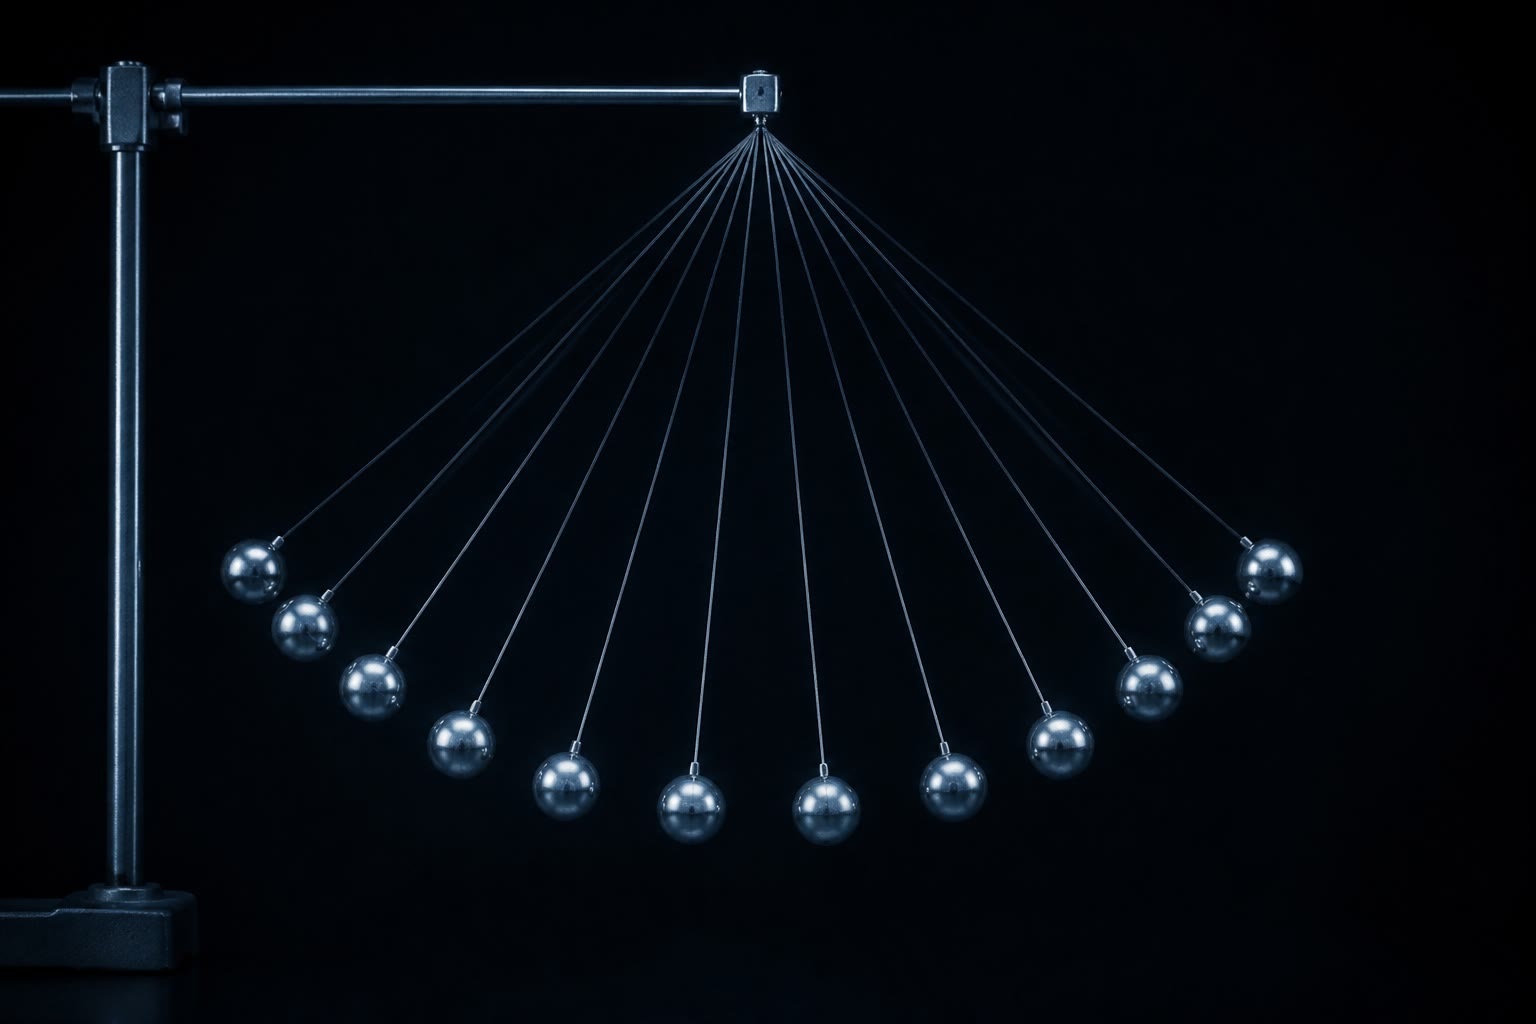
\includegraphics[width=0.58\linewidth]{images/book5/ai/b5-02-pendulum-strobe.jpg}

{\small Un péndulo fotografiado con luz estroboscópica: las posiciones se apiñan cerca de los puntos de retorno, donde la lenteja se demora, y se separan abajo, donde se apresura --- una fotografía del retrato en el \omterm{def:b3:hamiltonian-mechanics:hamiltonian}{espacio de fases} que este capítulo dibuja con ecuaciones.}
\end{omfigure}

\section{Ejercicios}

\begin{exercise}[$\star$]\label{exo:b3:hamiltonian-mechanics:1}
Para la masa sujeta al resorte: (a) constrúyase $H$ a partir de $L$ y
compruébese que $H =
E_k + E_p$; (b) escríbanse las \omterm{def:b3:hamiltonian-mechanics:hamiltonian}{ecuaciones canónicas} y verifíquese que reproducen
$\ddot x = -\omega^2x$; (c) muéstrese que las trayectorias son elipses en el
plano $(x, p)$ y dense sus semiejes a la energía $E$; (d) ¿en qué sentido
recorre el punto representativo su trayectoria?
\end{exercise}

\begin{exercise}[$\star$]\label{exo:b3:hamiltonian-mechanics:2}
La cuenta sobre el aro que gira del capítulo anterior tiene $L =
\tfrac12 mR^2\dot\theta^2 + \tfrac12 m\omega^2R^2\sin^2\theta +
mgR\cos\theta$. (a) Calcúlense $p$ y $H$. (b) ¿Se conserva $H$? ¿Es la
energía mecánica? (c) Esbócense las curvas de nivel de $H$ para
$\omega^2 < g/R$ y $\omega^2 > g/R$, usando el potencial efectivo de aquel
capítulo. (d) Identifíquense los centros, los puntos de silla y las
separatrices en el caso rápido.
\end{exercise}

\begin{exercise}[$\star$]\label{exo:b3:hamiltonian-mechanics:3}
Una pelota rebota elásticamente en el suelo, $H = p^2/2m + mgz$ ($z >
0$). (a) Dibújense la trayectoria de fase de un vuelo y la del movimiento
completo de rebotes. (b) ¿Qué le hace el rebote elástico al punto
representativo? (c) Calcúlense el área encerrada para una altura máxima
$z_{\max}$ y la \omterm{def:b3:lagrangian-mechanics:action}{acción} $I$. (d) La regla de Bohr--Sommerfeld
$\oint p\,\dd z = nh$ aplicada a un neutrón que rebota ($m =
\qty{1.67e-27}{kg}$) da alturas de rebote cuantizadas: estímese la menor y
compárese con los \qty{15}{\micro m} medidos en el experimento de estados
cuánticos gravitatorios de 2002.
\end{exercise}

\begin{exercise}[$\star$]\label{exo:b3:hamiltonian-mechanics:4}
Solo a partir de las relaciones canónicas, calcúlese (a) $\{x^2, p\}$; (b)
$\{xp, H\}$ para $H = p^2/2m + E_p(x)$, e interprétense los dos términos
(este corchete rige el \emph{teorema del virial}); (c) $\{L_z, x\}$ y
$\{L_z, p_x\}$; (d) muéstrese que si $\{f, H\} = 0$ y $\{g, H\} = 0$
entonces $\{f, g\}$ también se conserva (úsese la identidad de Jacobi, que se
admite: $\{f,\{g,h\}\} + \{g,\{h,f\}\} + \{h,\{f,g\}\} = 0$).
\end{exercise}

\begin{exercise}[$\star\star$]\label{exo:b3:hamiltonian-mechanics:5}
El péndulo cerca de su \omterm{def:b3:hamiltonian-mechanics:portrait}{separatriz}. (a) Dese la energía de la \omterm{def:b3:hamiltonian-mechanics:portrait}{separatriz} y el
$|p|$ máximo sobre ella. (b) Muéstrese que sobre la \omterm{def:b3:hamiltonian-mechanics:portrait}{separatriz} $p =
\pm 2m\ell^2\omega_0\cos(\theta/2)$ con $\omega_0 = \sqrt{g/\ell}$.
(c) Usando $\dot\theta = p/m\ell^2$, muéstrese que el tiempo de ir de
$\theta$ a lo alto diverge logarítmicamente. (d) Un péndulo real soltado
justo por debajo de la \omterm{def:b3:hamiltonian-mechanics:portrait}{separatriz} permanece cerca de la posición invertida
durante un largo instante antes de volver --- relaciónese con (c) y con la
ralentización que se observa cerca de todo punto de silla.
\end{exercise}

\begin{exercise}[$\star\star$]\label{exo:b3:hamiltonian-mechanics:6}
Una partícula cargada en un campo magnético tiene $H = (\vect p -
q\vect A)^2/2m$, con $\vect p$ el momento canónico del capítulo
anterior. (a) Escríbanse las \omterm{def:b3:hamiltonian-mechanics:hamiltonian}{ecuaciones canónicas} para $\vect A = \tfrac12
B(-y, x, 0)$ y compruébese que dan el movimiento ciclotrónico. (b) Muéstrese
que $H =
\tfrac12 m\vect v^{\,2}$: el campo magnético no realiza trabajo. (c) Calcúlese
el corchete de las dos magnitudes conservadas $\pi_x = p_x - \tfrac12
qBy$ y $\pi_y = p_y + \tfrac12 qBx$ (compruébese antes que cada una se
conserva) y muéstrese que $\{\pi_x, \pi_y\} = -qB$: dos magnitudes
conservadas cuyo corchete es una constante. (d) Úsese el
\cref{exo:b3:hamiltonian-mechanics:4}(d) para explicar por qué no cabía
esperar de ellas una tercera magnitud conservada independiente.
\end{exercise}

\begin{exercise}[$\star\star$]\label{exo:b3:hamiltonian-mechanics:7}
Liouville, a mano. (a) Para la partícula libre, el flujo es $q \to q +
pt/m$, $p \to p$: muéstrese que un rectángulo se convierte en un
paralelogramo de la misma área. (b) Para el oscilador armónico, muéstrese
que el flujo es una rotación (en unidades adecuadas) y conclúyase. (c) Para el
oscilador \emph{amortiguado} $\ddot x = -\omega^2x - \gamma\dot x$, escríbase
la divergencia del flujo en el plano $(x, v)$ y muéstrese que las áreas se
contraen como $\eu^{-\gamma t}$: el amortiguamiento no es \omterm{def:b3:hamiltonian-mechanics:hamiltonian}{hamiltoniano}.
(d) ¿Adónde ``va'' físicamente el área perdida?
\end{exercise}

\begin{exercise}[$\star\star$]\label{exo:b3:hamiltonian-mechanics:8}
Movimiento plano en un potencial central, $H = (p_r^2 + p_\varphi^2/r^2)/2m
+ E_p(r)$. (a) Escríbanse las cuatro \omterm{def:b3:hamiltonian-mechanics:hamiltonian}{ecuaciones canónicas}. (b) Muéstrese que $\{
p_\varphi, H\} = 0$ e identifíquese la ley de conservación. (c) Redúzcase a un
\omterm{def:b3:hamiltonian-mechanics:hamiltonian}{hamiltoniano} radial unidimensional con un potencial efectivo. (d) Para
$E_p = -k/r$, localícese la órbita circular con $p_\varphi$ dado y dese su
energía --- que se cuantizará en el
\cref{pb:b3:hamiltonian-mechanics:1}.
\end{exercise}

\begin{exercise}[$\star\star$]\label{exo:b3:hamiltonian-mechanics:9}
(a) Verifíquese $\{L_x, L_y\} = L_z$ a partir de las relaciones canónicas.
(b) Dedúzcanse los otros dos corchetes por permutación cíclica. (c) Muéstrese
que $\{L^2, L_z\} = 0$. (d) Un sólido rígido gira libremente: tomando $H =
L^2/2J$ (inercia de simetría esférica), muéstrese que los tres $L_i$ se
conservan; ¿y para un cuerpo con momentos de inercia distintos (respóndase
cualitativamente a partir de los corchetes)?
\end{exercise}

\begin{exercise}[$\star\star\star$]\label{exo:b3:hamiltonian-mechanics:10}
Niveles de la vieja teoría cuántica. (a) Muéstrese que $\oint p\,\dd q = nh$
aplicada al oscilador armónico da $E_n = n\hbar\omega$, usando la
\cref{prop:b3:hamiltonian-mechanics:sho-action}. (b) Aplíquese a la
partícula en una caja de longitud $a$ y recupérese exactamente $E_n =
n^2h^2/8ma^2$. (c) Para una molécula diatómica modelizada como un oscilador
de rigidez $k = \qty{1.9e3}{N/m}$ y masa reducida $\qty{1.14e-26}
{kg}$ (monóxido de carbono), calcúlese $\hbar\omega$ en eV y la longitud de
onda de la emisión $n = 1 \to 0$; ¿en qué rango espectral cae? (d) Los
niveles verdaderos son $(n + \tfrac12)\hbar\omega$: ¿cambia ese medio que
falta las longitudes de onda \emph{emitidas}? ¿Qué experimento sí detecta
el medio del punto cero?
\end{exercise}

\begin{exercise}[$\star\star\star$]\label{exo:b3:hamiltonian-mechanics:11}
Invariancia adiabática de $E/\omega$, deducida. Una masa sujeta a un resorte
cuya rigidez $k(t)$ crece lentamente. (a) Muéstrese que $\dot E = \tfrac12\dot k\,
x^2$ a lo largo del movimiento exacto. (b) Promédiese sobre un periodo con $k$
fija: usando $\langle\tfrac12 kx^2\rangle = E/2$, muéstrese que $\langle\dot E\rangle
= \dot k\,E/2k$. (c) Conclúyase que $\dd\ln E = \tfrac12\dd\ln k = \dd\ln
\omega$, luego $E/\omega$ es constante. (d) Un péndulo que oscila con
amplitud $\theta_0 = 5^\circ$ ve su cuerda acortada lentamente de
\qty{1.0}{m} a \qty{0.5}{m}: hállense la nueva amplitud y el factor en que
creció su energía, y dígase de dónde salió esa energía.
\end{exercise}

\begin{exercise}[$\star\star\star$]\label{exo:b3:hamiltonian-mechanics:12}
El área encerrada por la \omterm{def:b3:hamiltonian-mechanics:portrait}{separatriz} del péndulo es un número de estados
cuánticos. (a) Muéstrese que $\oint p\,\dd\theta$ a lo largo de la
\omterm{def:b3:hamiltonian-mechanics:portrait}{separatriz} vale $16m\ell^2\omega_0$. (b) Por la regla de Bohr--Sommerfeld,
el número de estados cuánticos con energía por debajo de la \omterm{def:b3:hamiltonian-mechanics:portrait}{separatriz} es
$N \approx
16m\ell^2\omega_0/h$: evalúese para una masa de un gramo con una cuerda de
\qty{10}{cm}. (c) Evalúese para un oscilador molecular tipo amoniaco:
$m \sim \qty{1e-26}{kg}$, $\ell \sim \qty{1e-10}{m}$,
$\omega_0 \sim \qty{1e14}{rad/s}$. (d) Conclúyase: ¿dónde está la frontera
entre la mecánica que necesita $\hbar$ y la que no lo necesita?
\end{exercise}

\section{Problema: la vieja teoría cuántica y el átomo de hidrógeno}

\begin{problem}[{Problema de fin de semana --- cuantizar el espacio de
fases, pesar el Rydberg}]\label{pb:b3:hamiltonian-mechanics:1}
En 1913 Bohr calculó el espectro del hidrógeno a partir de la mecánica
planetaria más una regla cuántica; Sommerfeld reconoció en esa regla un
enunciado sobre el área del \omterm{def:b3:hamiltonian-mechanics:hamiltonian}{espacio de fases}. Este problema reconstruye su
cálculo con las herramientas de este capítulo. Datos: $m_{\text{e}} =
\qty{9.11e-31}{kg}$, $e = \qty{1.60e-19}{C}$, $1/4\pi\varepsilon_0 =
\qty{8.99e9}{N.m^2/C^2}$, $h = \qty{6.63e-34}{J.s}$, $c =
\qty{3.00e8}{m/s}$. Escribimos $k = e^2/4\pi\varepsilon_0$.

\medskip\noindent\textbf{Parte I --- El \omterm{def:b3:hamiltonian-mechanics:hamiltonian}{hamiltoniano} de Kepler.}
Un electrón se mueve en el plano alrededor de un protón fijo.
\begin{enumerate}
  \item Justifíquese que se trate el protón como fijo (razón de masas) y
        escríbase el \omterm{def:b3:hamiltonian-mechanics:hamiltonian}{hamiltoniano} $H = \dfrac{p_r^2}{2m_{\text{e}}} +
        \dfrac{p_\varphi^2}{2m_{\text{e}}r^2} - \dfrac{k}{r}$.
  \item Escríbanse las cuatro \omterm{def:b3:hamiltonian-mechanics:hamiltonian}{ecuaciones canónicas}.
  \item Muéstrese que $p_\varphi$ se conserva y dese nombre.
  \item Redúzcase el movimiento radial al potencial efectivo
        $U_{\text{ef}}(r) = p_\varphi^2/2m_{\text{e}}r^2 - k/r$ y
        esbócese.
  \item Localícese la órbita circular: $r_{\text{c}} =
        p_\varphi^2/m_{\text{e}}k$.
  \item Muéstrese que su energía es $E = -k/2r_{\text{c}} =
        -m_{\text{e}}k^2/2p_\varphi^2$ y compruébese que es la mitad de la
        energía potencial (la razón del virial de las órbitas
        gravitatorias del volumen del Año 1).
\end{enumerate}

\medskip\noindent\textbf{Parte II --- La órbita clásica.}
\begin{enumerate}[resume]
  \item Para una órbita circular de radio $r$, hállese la velocidad $v$ y la
        frecuencia orbital $f_{\text{orb}}$ en función de $r$.
  \item Una órbita de tamaño atómico, $r = \qty{0.05}{nm}$: calcúlese $v$
        (y $v/c$), $f_{\text{orb}}$ y la energía en eV.
  \item Calcúlese el momento angular $p_\varphi$ de esa órbita y
        compárese con $\hbar = h/2\pi$: ¿qué sugiere la coincidencia?
  \item Clásicamente, un electrón en órbita es un dipolo oscilante y
        radia (volumen del Año 2) a $f_{\text{orb}}$; su energía decae
        en unos \qty{1e-11}{s}. Enúnciense las dos predicciones fatales
        que esto hace para los átomos y qué se observa en su lugar.
  \item ¿Qué rasgo de los espectros observados (líneas discretas, regla
        de combinación $1/\lambda = R_H(1/n^2 - 1/n'^2)$) sugirió
        \emph{niveles} discretos de energía?
  \item Explíquese por qué un \emph{\omterm{prop:b3:hamiltonian-mechanics:adiabatic}{invariante adiabático}} es el candidato
        natural a magnitud que toma valores universales fijos
        (recuérdese la \cref{prop:b3:hamiltonian-mechanics:adiabatic}).
\end{enumerate}

\medskip\noindent\textbf{Parte III --- Cuantización.}
Impóngase la regla de Sommerfeld al movimiento angular de la órbita
circular: $\oint p_\varphi\,\dd\varphi = nh$, $n = 1, 2, 3, \dots$
\begin{enumerate}[resume]
  \item Muéstrese que la regla se lee $p_\varphi = n\hbar$.
  \item Dedúzcanse los radios permitidos $r_n = n^2a_0$ con $a_0 =
        \hbar^2/m_{\text{e}}k$, y calcúlese $a_0$.
  \item Dedúzcanse las energías permitidas $E_n = -E_{\text{I}}/n^2$ con
        $E_{\text{I}} = m_{\text{e}}k^2/2\hbar^2$, y calcúlese
        $E_{\text{I}}$ en julios y en eV.
  \item Calcúlese la velocidad en la primera órbita y compruébese que $v_1/c =
        k/\hbar c \approx 1/137$ (la constante de estructura fina).
  \item Un fotón se lleva la energía de una transición: dedúzcanse la
        fórmula de Rydberg y el valor de $R_H = E_{\text{I}}/hc$;
        compárese con los \qty{1.097e7}{m^{-1}} medidos.
  \item Calcúlense las longitudes de onda de las transiciones $2 \to 1$,
        $3 \to 2$ e $\infty \to 2$; ¿cuál es visible y de qué color?
  \item El ion de helio ionizado He$^+$ es un hidrógeno con carga nuclear
        $2e$: ¿cómo escalan $a_0$ y $E_{\text{I}}$, y dónde cae
        su línea $2 \to 1$?
\end{enumerate}

\medskip\noindent\textbf{Parte IV --- Confrontación.}
\begin{enumerate}[resume]
  \item Calcúlese la frecuencia orbital $f_{\text{orb}}(n)$ y la
        frecuencia de transición $\nu_{n \to n-1}$ para $n = 2$, $10$,
        $100$, y muéstrese que su cociente tiende a $1$ al crecer $n$.
  \item Este es el \emph{principio de correspondencia} de Bohr:
        enúnciese en una frase.
  \item La regla $p_\varphi = n\hbar$ empieza en $n = 1$: ¿qué absurdo
        significaría $n = 0$ para una órbita circular?
  \item La mecánica cuántica conservará exactamente $E_n = -E_{\text{I}}/n^2$,
        pero descartará las órbitas: nómbrense dos hechos medibles que la
        imagen orbital predice mal (el valor del momento angular del
        estado fundamental y la existencia de estados con el mismo $n$ y
        formas distintas).
  \item El muon es un electrón $207$ veces más pesado: para el hidrógeno
        muónico, calcúlense $a_0^\mu$ y $E_{\text{I}}^\mu$, y explíquese por
        qué los átomos muónicos sondean el \emph{núcleo}.
  \item Resúmase el resultado con nombre propio: un \omterm{prop:b3:hamiltonian-mechanics:adiabatic}{invariante adiabático},
        igualado a números enteros de $h$, produce $a_0 = \qty{52.9}{pm}$,
        $E_{\text{I}} = \qty{13.6}{eV}$ y el espectro del hidrógeno con
        cuatro cifras --- y entrega a la teoría verdadera sus dos
        constantes centrales.
\end{enumerate}
\end{problem}
